%!TEX TS-program = xelatex
\documentclass[12pt, a4paper, oneside]{article}

\usepackage{amsmath,amsfonts,amssymb,amsthm,mathtools}  % пакеты для математики

\usepackage[utf8]{inputenc} % задание utf8 кодировки исходного tex файла
\usepackage[british,russian]{babel} % выбор языка для документа

\usepackage{fontspec}         % пакет для подгрузки шрифтов
\setmainfont{Helvetica}   % задаёт основной шрифт документа

% why do we need \newfontfamily:
% http://tex.stackexchange.com/questions/91507/
\newfontfamily{\cyrillicfonttt}{Helvetica}
\newfontfamily{\cyrillicfont}{Helvetica}
\newfontfamily{\cyrillicfontsf}{Helvetica}

\usepackage{unicode-math}     % пакет для установки математического шрифта
\setmathfont{Neo Euler}      % шрифт для математики
% \setmathfont[math-style=ISO]{Asana Math}
% Можно делать смену начертания с помощью разных стилей

% Конкретный символ из конкретного шрифта
% \setmathfont[range=\int]{Neo Euler}

%%%%%%%%%% Работа с картинками %%%%%%%%%
\usepackage{graphicx}                  % Для вставки рисунков
\usepackage{graphics}
\graphicspath{{images/}{pictures/}}    % можно указать папки с картинками
\usepackage{wrapfig}                   % Обтекание рисунков и таблиц текстом

%%%%%%%%%%%%%%%%%%%%%%%% Графики и рисование %%%%%%%%%%%%%%%%%%%%%%%%%%%%%%%%%
\usepackage{tikz, pgfplots}  % язык для рисования графики из latex'a

%%%%%%%%%% Гиперссылки %%%%%%%%%%
\usepackage{xcolor}              % разные цвета

\usepackage{hyperref}
\hypersetup{
	unicode=true,           % позволяет использовать юникодные символы
	colorlinks=true,       	% true - цветные ссылки, false - ссылки в рамках
	urlcolor=blue,          % цвет ссылки на url
	linkcolor=red,          % внутренние ссылки
	citecolor=green,        % на библиографию
	pdfnewwindow=true,      % при щелчке в pdf на ссылку откроется новый pdf
	breaklinks              % если ссылка не умещается в одну строку, разбивать ли ее на две части?
}


\usepackage{todonotes} % для вставки в документ заметок о том, что осталось сделать
% \todo{Здесь надо коэффициенты исправить}
% \missingfigure{Здесь будет Последний день Помпеи}
% \listoftodos --- печатает все поставленные \todo'шки

\usepackage{enumitem} % дополнительные плюшки для списков
%  например \begin{enumerate}[resume] позволяет продолжить нумерацию в новом списке

\usepackage[paper=a4paper, top=20mm, bottom=15mm,left=20mm,right=15mm]{geometry}
\usepackage{indentfirst}       % установка отступа в первом абзаце главы

\usepackage{setspace}
\setstretch{1.15}  % Межстрочный интервал
\setlength{\parskip}{4mm}   % Расстояние между абзацами
% Разные длины в латехе https://en.wikibooks.org/wiki/LaTeX/Lengths


\usepackage{xcolor} % Enabling mixing colors and color's call by 'svgnames'

\definecolor{MyColor1}{rgb}{0.2,0.4,0.6} %mix personal color
\newcommand{\textb}{\color{Black} \usefont{OT1}{lmss}{m}{n}}
\newcommand{\blue}{\color{MyColor1} \usefont{OT1}{lmss}{m}{n}}
\newcommand{\blueb}{\color{MyColor1} \usefont{OT1}{lmss}{b}{n}}
\newcommand{\red}{\color{LightCoral} \usefont{OT1}{lmss}{m}{n}}
\newcommand{\green}{\color{Turquoise} \usefont{OT1}{lmss}{m}{n}}

\usepackage{titlesec}
\usepackage{sectsty}
%%%%%%%%%%%%%%%%%%%%%%%%
%set section/subsections HEADINGS font and color
\sectionfont{\color{MyColor1}}  % sets colour of sections
\subsectionfont{\color{MyColor1}}  % sets colour of sections

%set section enumerator to arabic number (see footnotes markings alternatives)
\renewcommand\thesection{\arabic{section}.} %define sections numbering
\renewcommand\thesubsection{\thesection\arabic{subsection}} %subsec.num.

%define new section style
\newcommand{\mysection}{
	\titleformat{\section} [runin] {\usefont{OT1}{lmss}{b}{n}\color{MyColor1}} 
	{\thesection} {3pt} {} } 


%	CAPTIONS
\usepackage{caption}
\usepackage{subcaption}
%%%%%%%%%%%%%%%%%%%%%%%%
\captionsetup[figure]{labelfont={color=Turquoise}}

\usepackage[normalem]{ulem}  % для зачекивания текста

\pagestyle{empty}

\begin{document}

\section*{Задание 6 (куча баллов)  }

Не забывай, где находится  \href{https://fulyankin.github.io/LaTeX/}{страничку курса} с кучей шпаргалок! А также где лежит \href{https://docs.google.com/forms/d/e/1FAIpQLSe11kxKVfv07iCL1E9yNX7ll9swKImiVwRr1H70lslGzInRSg/viewform}{уютная гугл-форма.} Не стесняйтесь просить о помощи, если она вам необходима.

\section*{Полезные задачи}

Пришло время заняться связкой R+LaTeX! Я настоятельно рекомендую как следует апробировать её. На мой взгляд, этот довольно полезный навык в ряде случаев может очень сильно упростить вам жизнь.

\subsection*{[20] Упражнение 1 (Карточки)}

Приближается контрольная работа по дискретной математике! Вам выпала честь составить огромное количество разнообразных вариантов для решения. У вас есть  \href{https://github.com/FUlyankin/LaTeX/tree/master/Logi_2018/Homework_2018/hw_7_baza_zadach.zip}{база данных из 4 различных типов задач.}   В каждом файле находится какое-то количество задач своего типа. В первом на элементарную комбинаторику, во втором на бином Ньютона, в третьем на формулу включений-исключений, в четвёртом на рекуррентные соотношения.

Нужно в связке R + \LaTeX{} написать скрипт, который сгенерирует максимальное количество вариантов контрольной работы так, чтобы:

\begin{itemize}
\item Каждый вариант контрольной генерировался случайно
\item Задачи в разных вариантах не повторялись
\item В каждом варианте должно быть две задачи на элементарную комбинаторику, одна задача на бином, одна задача на формулу включений-исключений и одна задача на рекурентные соотношения.
\end{itemize}

Все варианты контрольной работы должны быть записаны в один pdf-файл. Каждый вариант должен начинаться с новой страницы. Количество задач по разным темам различается. Все лишние задачи должны быть записаны в отдельный pdf-файл. Каждая в свою тематику. То есть на выход идёт два pdf-файла!


\subsection*{[10]  Упражнение 2}

Придумайте свой полезный скрипт, который будет выполнять какую-то работу в связке R + \LaTeX{}. Не забудьте подробно расписать какую именно проблему призван решить ваш скрипт и как именно он решает её.

\section*{Не очень полезные задачи}

\subsection*{[10]  Упражнение 3}

Cowsay — это настраиваемая говорящая и думающая корова! Эта\href{http://citkit.ru/articles/679/}{великая программа} была когда-то написана на Perl и с тех пор не может покинуть многие великие умы.

Если вы используете Linux, то вы можете поставить cowsay, прописав \texttt{sudo apt-get install cowsay}. После попробуйте ввести \texttt{cowsay Hello, World!}. Если у вас Mac, вы можете сделать всё то же самое через `brew`. Если у вас Windows, то побаловаться с коровой будет не очень просто. Не забудьте вернуться назад, в наш бренный мир, после экстаза, который вы испытаете!

\begin{center}
	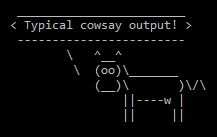
\includegraphics[scale=1]{Cowsay_Typical_Output.png}
\end{center}

\begin{itemize}
	\item Создайте в LaTeX своё окружение, которое будет работать по аналогии с cowsay. Нарисуйте все необходимые для него кусочки в Tikz. Можете использовать для этого Geogebra или уже готовые заготовки, которые вы найдёте на просторах интернета. Оригинальные ходы будут щедро поощрены.
	
	\item Модернизируйте окружение cowsay, написанное вами. Заставьте его при каждом новом обращении выдавать какую-нибудь рандомную мудрую фразу из заранее созданной базы данных. Каждый день в течение недели используйте этот скрипт перед завтраком.
\end{itemize}


\subsection*{[10]  Упражнение 4}

Диплом должен состоять из многих частей. Как минимум из трёх глав. А ещё в нём может быть куча приложений. Довольно удобно каждую главу писать в отдельном файле, а после собирать всё в единое целое. Напишите в связке R + \LaTeX{} скрипт, который соберёт вам готовый диплом из разных кусочков и удалит из папки весь мусор.

Никогда не пользуйтесь этим скриптом, потому что это немного странно и неудобно.


\subsection*{[10] Упражнение 5}

Часто возникают ситуации, когда отсканировано довольно много рисунков и из них нужно сверстать pdf-файл. Напишите в связке R + \LaTeX{} скрипт, который будет создавать из кучи рисунков красивый pdf-файл.

Никогда не пользуйтесь этим скриптом. Есть же удобные приложения, лол. На линуксе и маке это одна команда в терминале.

\section*{Хардкорные задачи}

\subsection*{[1000] Упражнение 6 (Настоящий шрифт вымогателя)}

Во втором домашнем задании вам было предложено написать письмо с угрозами. Для того, чтобы написать его, вы использовали шрифт вымогателей. Однако это не очень хороший шрифт вымогателей. Каждой букве "А", написанной таким шрифтом, соответствует одно единственное начертание. Когда вымогатели составляют реальные письма с угрозами, они вырезают из журналов большое количество различных букв "А". Вам предлагается решить эту проблему.

Напишите в связке R + \LaTeX{} скрипт, который будет генерировать письмо с угрозами так, что каждая новая буква будет иметь случайное начертание. Можно попробовать сделать это по заранее собранной базе с буквами. В таком случае для каждой буквы у вас будет конечное число написаний. Можно попробовать сделать макет буквы в TikZ и там же прописать правила её зашумления, чтобы при каждой генерации она выглядела по новому.
\end{document}
